
%(BEGIN_QUESTION)
% Copyright 2011, Tony R. Kuphaldt, released under the Creative Commons Attribution License (v 1.0)
% This means you may do almost anything with this work of mine, so long as you give me proper credit

This split-ranged valve system uses {\it 4-20 mA isolators} to drive identical current signals to each of three progressively split-ranged control valves, because the PLC's analog output card does not produce enough voltage to successfully power all three valve positioners if connected in series:

$$\includegraphics[width=15.5cm]{i01455x01.eps}$$

Unfortunately, this system has a problem.  When the PLC attempts to drive an output signal of 70\%, FV-101a is wide open, FV-101b is 86\% open, and FV-101c is 20\% open.

Determine the diagnostic value of each of the following tests.  Assume only one fault in the system, including any single component or any single wire/cable/tube connecting components together.  If a proposed test could provide new information to help you identify the location and/or nature of the one fault, mark ``yes.''  Otherwise, if a proposed test would not reveal anything relevant to identifying the fault (already discernable from the measurements and symptoms given so far), mark ``no.''

% No blank lines allowed between lines of an \halign structure!
% I use comments (%) instead, so that TeX doesn't choke.

$$\vbox{\offinterlineskip
\halign{\strut
\vrule \quad\hfil # \ \hfil & 
\vrule \quad\hfil # \ \hfil & 
\vrule \quad\hfil # \ \hfil \vrule \cr
\noalign{\hrule}
%
% First row
{\bf Diagnostic test} & {\bf Yes} & {\bf No} \cr
%
\noalign{\hrule}
%
% Another row
Check main air supply pressure gauge indication &  &  \cr
%
\noalign{\hrule}
%
% Another row
Check FV-101a positioner supply pressure gauge indication &  &  \cr
%
\noalign{\hrule}
%
% Another row
Check FV-101b positioner supply pressure gauge indication &  &  \cr
%
\noalign{\hrule}
%
% Another row
Check FV-101c positioner supply pressure gauge indication &  &  \cr
%
\noalign{\hrule}
%
% Another row
Measure DC current at PLC output card terminals &  &  \cr
%
\noalign{\hrule}
%
% Another row
Measure DC current at FV-101a positioner terminals &  &  \cr
%
\noalign{\hrule}
%
% Another row
Measure DC current at FV-101b positioner terminals &  &  \cr
%
\noalign{\hrule}
%
% Another row
Measure DC current at FV-101c positioner terminals &  &  \cr
%
\noalign{\hrule}
} % End of \halign 
}$$ % End of \vbox


\filbreak

\vskip 20pt \vbox{\hrule \hbox{\strut \vrule{} {\bf Suggestions for Socratic discussion} \vrule} \hrule}

\begin{itemize}
\item{} A problem-solving technique useful for making proper connections in pictorial circuit diagrams is to first identify the directions of all DC currents entering and exiting component terminals, as well as the respective voltage polarity marks (+,$-$) for those terminals, based on your knowledge of each component acting either as an electrical {\it source} or an electrical {\it load}.  Discuss and compare how these arrows and polarity marks simplify the task of properly connecting wires between components. 
\end{itemize}

\underbar{file i01455}
%(END_QUESTION)





%(BEGIN_ANSWER)

\noindent
{\bf Partial answer:}

% No blank lines allowed between lines of an \halign structure!
% I use comments (%) instead, so that TeX doesn't choke.

$$\vbox{\offinterlineskip
\halign{\strut
\vrule \quad\hfil # \ \hfil & 
\vrule \quad\hfil # \ \hfil & 
\vrule \quad\hfil # \ \hfil \vrule \cr
\noalign{\hrule}
%
% First row
{\bf Diagnostic test} & {\bf Yes} & {\bf No} \cr
%
\noalign{\hrule}
%
% Another row
Check main air supply pressure gauge indication &  &  \cr
%
\noalign{\hrule}
%
% Another row
Check FY-101a positioner supply pressure gauge indication &  & $\surd$ \cr
%
\noalign{\hrule}
%
% Another row
Check FY-101b positioner supply pressure gauge indication &  &  \cr
%
\noalign{\hrule}
%
% Another row
Check FY-101c positioner supply pressure gauge indication &  &  \cr
%
\noalign{\hrule}
%
% Another row
Measure DC current at PLC output card terminals &  & $\surd$ \cr
%
\noalign{\hrule}
%
% Another row
Measure DC current at FV-101a positioner terminals &  &  \cr
%
\noalign{\hrule}
%
% Another row
Measure DC current at FV-101b positioner terminals &  &  \cr
%
\noalign{\hrule}
%
% Another row
Measure DC current at FV-101c positioner terminals &  &  \cr
%
\noalign{\hrule}
} % End of \halign 
}$$ % End of \vbox

%(END_ANSWER)





%(BEGIN_NOTES)

% No blank lines allowed between lines of an \halign structure!
% I use comments (%) instead, so that TeX doesn't choke.

$$\vbox{\offinterlineskip
\halign{\strut
\vrule \quad\hfil # \ \hfil & 
\vrule \quad\hfil # \ \hfil & 
\vrule \quad\hfil # \ \hfil \vrule \cr
\noalign{\hrule}
%
% First row
{\bf Diagnostic test} & {\bf Yes} & {\bf No} \cr
%
\noalign{\hrule}
%
% Another row
Check main air supply pressure gauge indication &  & $\surd$ \cr
%
\noalign{\hrule}
%
% Another row
Check FY-101a positioner supply pressure gauge indication &  & $\surd$ \cr
%
\noalign{\hrule}
%
% Another row
Check FY-101b positioner supply pressure gauge indication & $\surd$ &  \cr
%
\noalign{\hrule}
%
% Another row
Check FY-101c positioner supply pressure gauge indication &  & $\surd$ \cr
%
\noalign{\hrule}
%
% Another row
Measure DC current at PLC output card terminals &  & $\surd$ \cr
%
\noalign{\hrule}
%
% Another row
Measure DC current at FV-101a positioner terminals &  & $\surd$ \cr
%
\noalign{\hrule}
%
% Another row
Measure DC current at FV-101b positioner terminals & $\surd$ &  \cr
%
\noalign{\hrule}
%
% Another row
Measure DC current at FV-101c positioner terminals &  & $\surd$ \cr
%
\noalign{\hrule}
} % End of \halign 
}$$ % End of \vbox


Control valve FV-101b is the only one not opening properly (it should be wide-open, along with FV-101a).  Therefore, it is only worthwhile to make measurements specific to that valve.








\filbreak \vskip 20pt \vbox{\hrule \hbox{\strut \vrule{} {\bf Virtual Troubleshooting} \vrule} \hrule}

\noindent
{\bf Predicting the effect of a given fault:} present each of the following faults to the students, one at a time, having them comment on all the effects each fault would produce.

\begin{itemize}
\item{} 
\item{} 
\item{} 
\end{itemize}


\vskip 10pt


\noindent
{\bf Identifying possible/impossible faults:} present symptoms to the students and then have them determine whether or not a series of suggested faults could account for all the symptoms, explaining {\it why} or {\it why not} for each proposed fault:

\begin{itemize}
\item{} Symptom: {\it }
\item{}  -- {\bf Yes/No}
\item{}  -- {\bf Yes/No}
\item{}  -- {\bf Yes/No}
\end{itemize}


\vskip 10pt


\noindent
{\bf Determining the utility of given diagnostic tests:} present symptoms to the students and then propose the following diagnostic tests one by one.  Students rate the value of each test, determining whether or not it would give useful information (i.e. tell us something we don't already know).  Students determine what different results for each test would indicate about the fault, if anything:

\begin{itemize}
\item{} Symptom: {\it FV-101C is wide-open all the time, even when the other valves stroke as they should}
\item{} Measure current signal out of PLC -- {\bf No}
\item{} Measure current signal out of FV-101C isolator -- {\bf Yes}
\item{} Check air supply pressure gauge -- {\bf No}
\item{} Measure AC supply voltage at FV-101C isolator -- {\bf No}
\item{} Push/pull flapper in FV-101C positioner -- {\bf Yes}
\end{itemize}


\vskip 10pt


\noindent
{\bf Diagnosing a fault based on given symptoms:} imagine the ??? fails ??? in this system (don't reveal the fault to students!).  Present the operator's observation(s) to the students, have them consider possible faults and diagnostic strategies, and then tell them the results of tests they propose based on the following symptoms, until they have properly identified the nature and location of the fault:

\begin{itemize}
\item{} Operator observation: {\it }
\item{} 
\item{} 
\end{itemize}















\vfil \eject

\noindent
{\bf Summary Quiz:}

Identify one practical reason for using {\it loop isolator} modules on 4-20 mA controller output loop circuits.

\begin{itemize}
\item{} The isolators reduce electric shock hazard to instrument technicians
\vskip 5pt 
\item{} The presence of one becomes an ideal lock-out point for worker safety
\vskip 5pt 
\item{} The isolator boosts the voltage available to drive final control elements
\vskip 5pt 
\item{} Less explosion hazard is present if an isolator provides power to the valve
\vskip 5pt 
\item{} Process noise is completely filtered out by each isolator module
\vskip 5pt 
\item{} Custom split-range calibrations may be easily implemented in the isolators
\end{itemize}


%INDEX% Troubleshooting review: electric circuit diagnostic test usefulness

%(END_NOTES)


